\documentclass[11pt]{article}

\usepackage[a4paper,margin=1in]{geometry}
\usepackage{enumitem}
\usepackage{graphicx}
\usepackage{helvet}
\usepackage{xcolor}
\usepackage{tabularray}
\usepackage{hyperref}
\usepackage{xurl}      % allow URLs to break at any character, avoids overfull hboxes
\usepackage{titlesec}
\usepackage{fvextra}   % better verbatim wrapping
\usepackage{tikz}
\usetikzlibrary{shapes.geometric, arrows.meta, positioning, fit, backgrounds, calc}

\UseTblrLibrary{booktabs}

% ---- Flowchart node/edge styles ----
\tikzset{
  base/.style={draw, rounded corners=2pt, minimum height=6.5mm, minimum width=15mm,
               font=\footnotesize, align=center, inner sep=3pt},
  agent/.style={base, fill=red!12,   draw=red!65!black},
  ext/.style={base,   fill=green!16,  draw=green!55!black},
  db/.style={base,    fill=blue!10,   draw=blue!65!black},
  io/.style={base,    fill=gray!10,   draw=gray!60},
  dec/.style={diamond, aspect=1.7, draw=gray!70, fill=gray!10,
              font=\scriptsize, align=center, inner sep=0pt, minimum size=9mm},
  fl/.style={-{Stealth[length=2mm]}, semithick, gray!55!black},
  lbl/.style={font=\scriptsize\itshape, fill=white, inner sep=1pt},
}

\hypersetup{colorlinks=true, urlcolor=blue, linkcolor=black}

% ---- Palette ----
\definecolor{headblue}{HTML}{1F3864}   % dark header fill
\definecolor{rowalt}{HTML}{EEF2F8}     % light zebra row
\definecolor{ruleblue}{HTML}{1F3864}

% ---- Section heading style ----
\titleformat{\section}{\normalfont\large\bfseries\color{ruleblue}}{\thesection.}{0.6em}{}
\titlespacing*{\section}{0pt}{1.4em}{0.6em}

\setlength{\parindent}{0pt}
\setlength{\parskip}{0.5em}

% ---- Reusable table styles ----
\SetTblrStyle{caption}{font=\bfseries}

\begin{document}

% =====================================================================
% Header block (Institute)
% =====================================================================
\begin{center}
    
\includegraphics[width=1.8cm]{logo.png}\\[6pt]
    {\Large\bfseries Indian Institute of Information Technology Una}\\[2pt]
    {\large\bfseries Himachal Pradesh}\\[2pt]
    (An Institute of National Importance under MoE)\\
    \textbf{Saloh, Una -177209}\\
    \href{http://www.iiitu.ac.in}{www.iiitu.ac.in}
\end{center}

{\color{ruleblue}\hrule height 1pt}
\vspace{2pt}
\hfill Date: 01 November, 2026

\begin{center}
    {\large\bfseries Review I}\\[2pt]
    {\large\bfseries Project Phase -- III (\textit{[CSL801]})}
\end{center}

% =====================================================================
% Identity table
% =====================================================================
\vspace{0.4em}
\begin{tblr}{
  width=\textwidth,
  colspec={Q[l,3cm] X[l] Q[l,3cm] X[l]},
  rowsep=4pt, colsep=8pt,
  cells={valign=m},
  column{1}={font=\bfseries}, column{3}={font=\bfseries},
  hlines={0.4pt,black}, vlines={0.4pt,black},
}
  Student Name & Nikhil Arora / Vishal Singh Bhadauriya / Shashank Sharma & Roll No. & 23140 / 23168 / 23154 \\
  Batch No. & \textit{43} & Semester & VII \\
  Branch & \textit{CSE} & Supervisor(s) & \textit{Dr. Shatrughan Modi} \\
\end{tblr}

% =====================================================================
% 1. Title
% =====================================================================
\section{Title of the Project}
Visper: An Autonomous On-Device Multimodal AI Assistant and Agentic Execution Engine for Android

% =====================================================================
% 2. Introduction
% =====================================================================
\section{Introduction}
Modern consumer AI assistants remain predominantly tethered to the cloud: every user query,
camera capture, and audio stream is transmitted to remote server farms for inference. This
architecture incurs substantial privacy risks through personal data exposure, creates absolute
reliance on high-bandwidth network connectivity, and introduces unpredictable latency.
While edge artificial intelligence has historically been constrained by mobile CPU and memory
limits, recent breakthroughs in 4-bit quantization (such as GGML/GGUF architectures) and
compact multimodal foundation models now make it feasible to host a fully autonomous,
zero-cloud multimodal assistant directly on commercial Android smartphones.

This project presents \textbf{Visper}, a completely offline, production-grade multimodal AI
assistant engineered for the Android platform. Visper transitions away from heavy, high-overhead
managed runtimes to a native C++ high-performance execution core (\texttt{llama.cpp}/GGML)
running as a localized sandboxed engine over loopback IPC. The system executes an optimized
multimodal language model (Qwen 3.5 0.8B quantized to \texttt{Q4\_K\_M}, $\sim$508\,MB)
coupled with a dedicated multimodal projector (\texttt{mmproj-F16}, $\sim$195\,MB), enabling
direct visual cross-attention reasoning over user images. To complement visual understanding,
an on-device Google ML Kit OCR pipeline is integrated for fine-grained handwriting and document
transcription. 

Beyond text and vision, Visper incorporates an end-to-end conversational voice loop featuring
bilingual speech recognition and low-latency, script-aware streaming text-to-speech (TTS) supporting
English, Hindi (\textit{Devanagari}), and Punjabi (\textit{Gurmukhi}), governed by grammatical
Subject-Object-Verb (SOV) prompt steering. Furthermore, the assistant acts as an agentic execution
engine capable of invoking safe hardware actions (flashlight control, system alarms, and
mathematical evaluations) and persisting an offline associative memory vault across sessions.
The entire application operates within an 800\,MB--1.1\,GB RAM footprint, fits into a compact
$\sim$30\,MB APK, and features an in-app resilient streaming model acquisition engine with
zero-restart auto-binding, benchmarked and verified on a 6\,GB RAM Android smartphone
(\textit{MediaTek Helio G96}).

% =====================================================================
% 3. Problem Definition
% =====================================================================
\section{Problem Definition}
Existing on-device mobile AI implementations and academic demonstrators suffer from four
fundamental architectural shortcomings:

\begin{itemize}[leftmargin=1.4em, itemsep=2pt]
    \item \textbf{High-overhead, fragile inference runtimes} -- Many existing mobile frameworks
    (such as early LiteRT-LM or MediaPipe GenAI solutions) carry excessive memory footprints,
    exhibit unstable lifecycle transitions on Android, or fail to support dynamic multi-target
    CPU vector optimizations (ARM NEON, FP16, and Dot Product) natively.
    \item \textbf{Fragmented multimodal perception} -- Existing mobile applications treat chat,
    computer vision (OCR), and voice input as disconnected silos rather than a unified
    cross-attention reasoning pipeline capable of interpreting visual tokens and spoken queries
    simultaneously without cloud intervention.
    \item \textbf{Linguistic and dialectal degradation in small models} -- Sub-1B quantized models
    typically suffer from severe English/Chinese tokenization bias. In Indic languages (such as
    Hindi and Punjabi), naive frequency and presence penalties severely penalize essential
    auxiliary verbs and postpositions (\textit{है, हैं, की, को, ਦਾ, ਦੀ}), resulting in broken
    sentence structures and awkward literal translations.
    \item \textbf{Passive text generation without device agency} -- Current assistants remain
    confined to text generation, lacking the agentic capability to parse user intent into
    actionable, safe device operations (hardware torch control, alarm setting, calculation)
    while maintaining private long-term associative memory across chat sessions.
    \item \textbf{Deployment and model acquisition friction} -- Edge AI projects commonly require
    cumbersome desktop ADB side-loading or manual file-system placement, lacking an in-app,
    resilient model acquisition mechanism that handles multi-hop CDN redirects with live telemetry.
\end{itemize}

The problem addressed by this project is the design, implementation, and empirical verification
of a unified, air-gapped Android platform that provides high-throughput multimodal intelligence,
conversational Indic voice interaction, agentic hardware control, and resilient self-contained
asset lifecycle management within a sub-1.2\,GB RAM constraint.

% =====================================================================
% 4. Objectives
% =====================================================================
\section{Objectives}
\begin{enumerate}[leftmargin=1.6em, itemsep=3pt]
    \item \textbf{Native on-device multimodal inference} -- Integrate a native C++ GGML/llama.cpp
    inference daemon running locally over loopback HTTP/SSE, executing Qwen 3.5 0.8B
    (\texttt{Q4\_K\_M}) with a companion \texttt{mmproj-F16} visual projector on Android 64-bit ARM.
    \item \textbf{Hardware-accelerated dynamic instruction dispatch} -- Package multi-variant
    native CPU backends targeting ARMv8.0-A up to ARMv9.2-A, dynamically selecting ARM NEON,
    Dot Product (\texttt{ASIMDDP}), and half-precision FP16 vector instructions at runtime.
    \item \textbf{Hybrid visual understanding \& document extraction} -- Build a two-stage vision
    pipeline combining direct visual cross-attention projection with on-device Google ML Kit Text
    Recognition (OCR) and PDF/plaintext document ingestion for grounded contextual reasoning.
    \item \textbf{Conversational voice \& Indic dialect engine} -- Implement offline voice input
    using Android's \texttt{SpeechRecognizer} adapted for bilingual recognition (Hindi, Punjabi,
    and English), paired with a low-latency streaming TTS engine (\texttt{VisperTtsManager})
    featuring dynamic script detection and Indic punctuation sentence boundary chunking.
    \item \textbf{Grammatical steering for Indic linguistic fluency} -- Eliminate token penalty
    traps and resolve Subject-Object-Verb (SOV / \textit{कर्ता-कर्म-क्रिया}) syntactic framing
    in Hindi and Punjabi through system prompt steering and calibrated sampling parameters
    ($\mathrm{temp}=0.3, \mathrm{top\_p}=0.85, \mathrm{penalties}=0.1$).
    \item \textbf{Safe agentic execution \& private memory vault} -- Implement a deterministic
    device action dispatcher (\texttt{DeviceActionManager}) for flashlight control, system alarms,
    and mathematical computations, coupled with an encrypted, offline associative memory store.
    \item \textbf{Resilient in-app model downloader} -- Engineer a streaming coroutine download
    manager supporting HTTP multi-hop redirect resolution (Hugging Face CloudFront CDN), atomic
    file assembly, real-time speed/ETA metrics, and zero-restart engine binding.
    \item \textbf{End-to-end hardware validation} -- Package an optimized $\sim$30\,MB APK and
    empirically benchmark token throughput, TTFT, thermals, and memory on a 6\,GB RAM smartphone
    (\textit{Redmi Note 11S / MediaTek Helio G96}).
\end{enumerate}

% =====================================================================
% 5. Skillset table
% =====================================================================
\section{Skillset additionally required to solve/address the problem}
\begin{tblr}{
  width=\textwidth,
  colspec={Q[l,4.5cm] X[l]},
  rowsep=4pt, colsep=8pt,
  cells={valign=m},
  row{1}={bg=headblue, fg=white, font=\bfseries},
  row{even}={bg=rowalt},
  column{1}={font=\bfseries},
  hlines={0.3pt,black!30}, vlines={0.3pt,black!30},
}
  Domain & Specific Skills to Acquire \\
  Native Android \& C++ NDK & Android NDK cross-compilation, CMake configuration for GGML, dynamic loading (\texttt{dlopen}), multi-target ABI filtering (\texttt{arm64-v8a}), and loopback IPC socket communication \\
  Edge Multimodal Architecture & GGUF tensor format specifications, multimodal projector token alignment (\texttt{mmproj}), image down-sampling, and cross-attention vision tokenization \\
  Linguistic \& Sampling Optimization & Token probability distribution tuning, frequency/presence penalty calibration for agglutinative/postpositional languages, SOV prompt engineering \\
  Speech \& Audio Engineering & Android \texttt{SpeechRecognizer} intent routing, error code 13 (missing language pack) mitigation, multi-language tagging, streaming TTS chunking with Indic danda (\textit{।}) regex \\
  Agentic Action Dispatch & Android \texttt{CameraManager} torch API, \texttt{AlarmManager} intents, deterministic regex command parsing, and isolated arithmetic evaluation \\
  Data Persistence & Local JSON/SQLite storage, multi-session metadata serialization, associative memory extraction, and encrypted preferences \\
  Reactive Mobile UI & Jetpack Compose declarative UI, Kotlin Coroutines, StateFlow architecture, real-time hardware telemetry inspection, and custom canvas rendering \\
  Resilient Network Engineering & Chunked streaming HTTP input streams, multi-hop 302/307 redirect resolution, atomic \texttt{.part} file staging, and download coroutine cancellation \\
\end{tblr}

% =====================================================================
% 6. Timeline to achieve the skillset
% =====================================================================
\section{Timeline to achieve the skillset}
The skillset was acquired through progressive, iterative milestones aligned directly with the
architectural evolution of the platform.

\begin{tblr}{
  width=\textwidth,
  colspec={Q[l,6cm] Q[c,2.4cm] X[l]},
  rowsep=4pt, colsep=8pt,
  cells={valign=m},
  row{1}={bg=headblue, fg=white, font=\bfseries},
  row{even}={bg=rowalt},
  hlines={0.3pt,black!30}, vlines={0.3pt,black!30},
}
  Skill Area & Learning Window & Approach \\
  Native NDK \& llama.cpp Integration & Weeks 1--2 & Cross-compiled GGML libraries, established local loopback HTTP daemon, benchmarked initial text inference \\
  Android Jetpack Compose UI Scaffolding & Weeks 2--3 & Engineered reactive chat interface, bottom sheets, telemetry badges, and permission management \\
  Multimodal Projector \& Vision Pipeline & Weeks 4--5 & Integrated \texttt{mmproj-F16}, visual token injection, and Google ML Kit OCR text recognition \\
  Audio STT \& Speech Error Handling & Weeks 5--6 & Configured \texttt{SpeechRecognizer}, eliminated SODA error 13 by removing rigid offline locks, enabled \texttt{hi-IN} / \texttt{pa-IN} \\
  Indic Dialect \& Streaming TTS Engine & Weeks 7--8 & Built \texttt{VisperTtsManager}, implemented script detection (Devanagari/Gurmukhi), added Indic punctuation chunking \\
  Linguistic Tuning \& SOV Prompt Steering & Weeks 8--9 & Calibrated sampling penalties to preserve Indic auxiliary verbs, established SOV grammatical steering \\
  Agentic Actions \& Associative Memory & Weeks 9--10 & Implemented \texttt{DeviceActionManager} for torch/alarm/math and engineered long-term \texttt{LocalMemoryStore} \\
  Resilient Model Downloader & Weeks 11--12 & Built HTTP redirect streaming downloader with atomic \texttt{.part} writing and live progress telemetry \\
  Profiling, Packaging \& Hardware Verification & Weeks 13--14 & Applied R8 shrinking, resolved memory leaks, assembled release APK, and verified performance on physical hardware \\
\end{tblr}

% =====================================================================
% 7. Block schematic / algorithm / metrics
% =====================================================================
\section{Block schematic / algorithm / coding / testing metrics / experiments / result graphs / technical papers}

Figure~\ref{fig:workflow} illustrates the unified end-to-end operational pipeline of Visper:
multimodal input capture (text, camera/gallery imagery, documents, or spoken voice), perception
pre-processing (OCR or bilingual speech recognition), context and memory augmentation, SOV
dialect steering, localized loopback IPC inference through the native GGML engine, deterministic
agentic action execution, and real-time streaming response delivery via text and audio.

\begin{figure}[htbp]
\centering
\resizebox{\textwidth}{!}{%
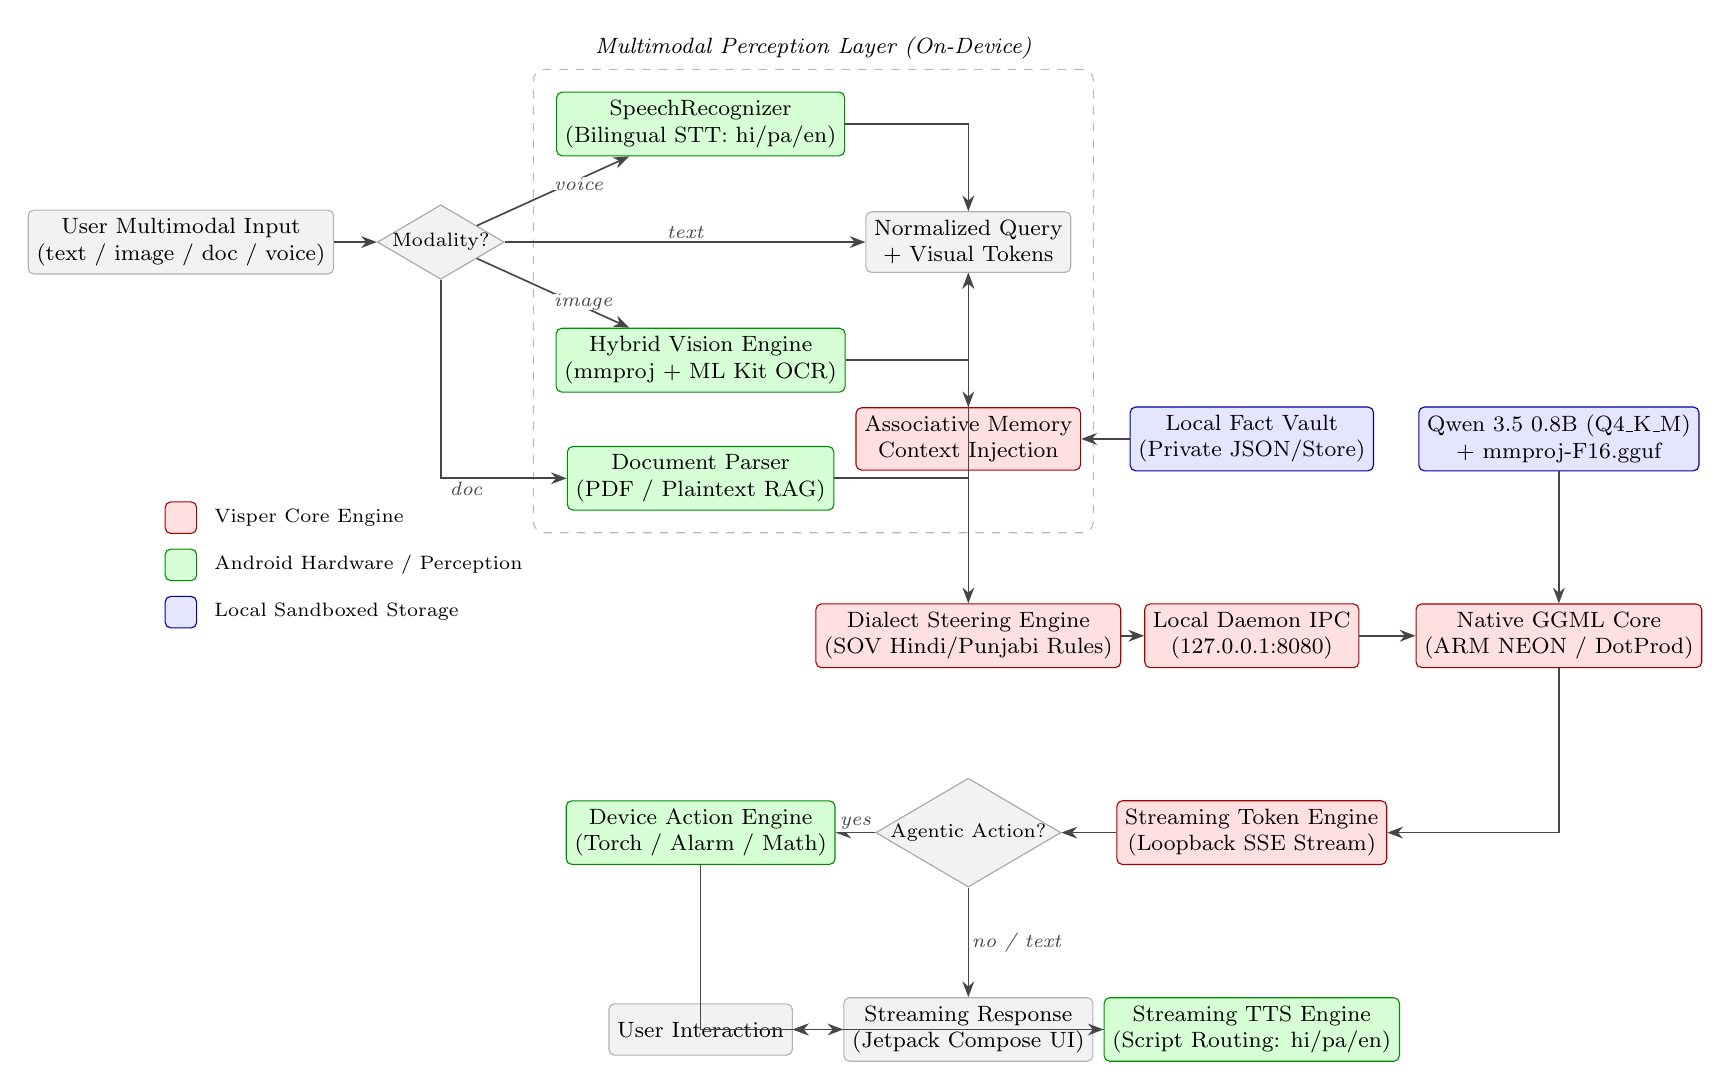
\begin{tikzpicture}[y=-1cm]  % y grows downward
  % ---- Input capture ----
  \node[io]  (input)  at (0,0)     {User Multimodal Input\\(text / image / doc / voice)};
  \node[dec] (mod)    at (3.3,0)   {Modality?};
  \node[ext] (stt)    at (6.6,-1.5){SpeechRecognizer\\(Bilingual STT: hi/pa/en)};
  \node[ext] (vision) at (6.6,1.5) {Hybrid Vision Engine\\(mmproj + ML Kit OCR)};
  \node[ext] (doc)    at (6.6,3.0) {Document Parser\\(PDF / Plaintext RAG)};
  \node[io]  (qtext)  at (10,0)    {Normalized Query\\+ Visual Tokens};

  % ---- Context & Memory ----
  \node[agent] (mem)  at (10,2.5)  {Associative Memory\\Context Injection};
  \node[db]    (db)   at (13.6,2.5){Local Fact Vault\\(Private JSON/Store)};

  % ---- Model orchestration & Prompt steering ----
  \node[agent] (orch) at (10,5.0)  {Dialect Steering Engine\\(SOV Hindi/Punjabi Rules)};
  \node[agent] (daemon) at (13.6,5.0){Local Daemon IPC\\(127.0.0.1:8080)};
  \node[agent] (ggml) at (17.5,5.0){Native GGML Core\\(ARM NEON / DotProd)};

  % ---- Model weights ----
  \node[db]    (weights) at (17.5,2.5){Qwen 3.5 0.8B (Q4\_K\_M)\\+ mmproj-F16.gguf};

  % ---- Inference + output ----
  \node[agent] (infer) at (13.6,7.5){Streaming Token Engine\\(Loopback SSE Stream)};
  \node[dec]   (act)   at (10,7.5)  {Agentic Action?};
  \node[ext]   (device)at (6.6,7.5) {Device Action Engine\\(Torch / Alarm / Math)};
  \node[io]    (resp)  at (10,10.0) {Streaming Response\\(Jetpack Compose UI)};
  \node[ext]   (tts)   at (13.6,10.0){Streaming TTS Engine\\(Script Routing: hi/pa/en)};
  \node[io]    (user2) at (6.6,10.0){User Interaction};

  % ---- Edges ----
  \draw[fl] (input) -- (mod);
  \draw[fl] (mod) -- node[lbl,above right,inner sep=0pt]{voice} (stt);
  \draw[fl] (mod) -- node[lbl,below right,inner sep=0pt]{image} (vision);
  \draw[fl] (mod) |- node[lbl,pos=0.6,below]{doc} (doc);
  \draw[fl] (mod) -- node[lbl,above]{text} (qtext);
  \draw[fl] (stt) -| (qtext);
  \draw[fl] (vision) -| (qtext);
  \draw[fl] (doc) -| (qtext);

  \draw[fl] (qtext) -- (mem);
  \draw[fl] (db) -- (mem);
  \draw[fl] (mem) -- (orch);

  \draw[fl] (orch) -- (daemon);
  \draw[fl] (daemon) -- (ggml);
  \draw[fl] (weights) -- (ggml);

  \draw[fl] (ggml) |- (infer);
  \draw[fl] (infer) -- (act);
  \draw[fl] (act) -- node[lbl,above]{yes} (device);
  \draw[fl] (act) -- node[lbl,right]{no / text} (resp);
  \draw[fl] (device) |- (resp);

  \draw[fl] (resp) -- (tts);
  \draw[fl] (resp) -- (user2);
  \draw[fl] (tts) -- (user2);

  % ---- Dashed container around input-capture cluster ----
  \begin{scope}[on background layer]
    \node[draw=gray!55, dashed, rounded corners, inner sep=8pt,
          fit=(stt)(vision)(doc)(qtext),
          label={[font=\footnotesize\itshape]above:Multimodal Perception Layer (On-Device)}] {};
  \end{scope}

  % ---- Legend ----
  \node[agent, minimum width=4mm, minimum height=4mm] (l1) at (0,3.5) {};
  \node[anchor=west, font=\scriptsize] at (0.3,3.5) {Visper Core Engine};
  \node[ext, minimum width=4mm, minimum height=4mm] (l2) at (0,4.1) {};
  \node[anchor=west, font=\scriptsize] at (0.3,4.1) {Android Hardware / Perception};
  \node[db, minimum width=4mm, minimum height=4mm] (l3) at (0,4.7) {};
  \node[anchor=west, font=\scriptsize] at (0.3,4.7) {Local Sandboxed Storage};
\end{tikzpicture}%
}
\caption{End-to-End Multimodal Execution Workflow of Visper}
\label{fig:workflow}
\end{figure}

\textbf{Block Schematic (Layered Architecture).} The software system is structured into four
isolated, highly cohesive architectural tiers:

\begin{BVerbatim}[fontsize=\small, frame=single, rulecolor=\color{ruleblue}]
+-----------------------------------------------------------------------------+
|                               UI / UX Layer                                 |
|  Jetpack Compose Reactive UI | Hardware Telemetry (tok/s, RAM, TTFT, Temp)  |
|  Modern Input Tray (Photo/Doc/Voice) | Conversational Orb | AI Lab Sheet    |
+-----------------------------------------------------------------------------+
                                      |
+-----------------------------------------------------------------------------+
|                      ViewModel & Orchestration Layer                        |
|  TerminalViewModel StateFlow | Session Manager | Local Memory Fact Store    |
|  SOV Grammatical Steering Engine | Resilient Model Download Manager         |
+-----------------------------------------------------------------------------+
                                      |
        +-----------------------------+-----------------------------+
        v                                                           v
+-------------------------------+           +---------------------------------+
|   Perception & Action Layer   |           |    Native Core Inference Tier   |
| Google ML Kit (On-Device OCR) |           | llama.cpp Native C++ Daemon     |
| Bilingual SpeechRecognizer    |           | Multi-Target ARM NEON/FP16/Dot  |
| Script-Aware TTS Engine       |           | Loopback IPC Server (127.0.0.1) |
| DeviceActionManager (Torch/   |<--SSE/JSON| Qwen 3.5 0.8B (Q4_K_M) Core     |
|   Alarm/Math Execution)       |           | mmproj-F16 Multimodal Projector |
+-------------------------------+           +---------------------------------+
\end{BVerbatim}

\textbf{Core Execution Algorithm.}
\begin{Verbatim}[fontsize=\small, frame=single, rulecolor=\color{ruleblue}]
1. INPUT: user_input (text | image_uri | document_uri | speech_audio)
2. IF user_input is speech_audio:
       target_locale <- resolveSpeechLocale(userPreferredLanguage, systemRegion)
       query_text    <- SpeechRecognizer.transcribe(audio, target_locale)
   ELIF user_input is image_uri:
       visual_tokens <- ImageProcessor.encodeBase64Jpeg(image_uri, maxDim=640)
       ocr_text      <- MLKitTextRecognizer.process(image_uri)
       query_text    <- combine(prompt, ocr_text, visual_tokens)
   ELIF user_input is document_uri:
       doc_text      <- DocumentParser.extractText(document_uri)
       query_text    <- buildGroundedContext(prompt, doc_text)
   ELSE:
       query_text    <- user_input

3. memory_context <- LocalMemoryStore.getRelevantFacts(query_text)
4. system_prompt  <- DialectSteering.applySOVRules(basePrompt, targetLanguage)
5. request_payload <- buildChatCompletionsJson(
       messages=[system_prompt, memory_context, query_text],
       temperature=0.30, top_p=0.85, freq_pen=0.10, pres_pen=0.10
   )

6. IF isActionCommand(query_text):
       action_result <- DeviceActionManager.execute(query_text) // Torch, Alarm, Math
       render(action_result)
       TTS.speak(action_result)
       EXIT

7. token_stream <- LlamaCppEngine.postStream("http://127.0.0.1:8080", request_payload)
8. FOR EACH token IN token_stream:
       UI.emitStreamingToken(token)
       TTSBuffer.append(token)
       IF TTSBuffer.matchesSentenceBoundary(Regex("(?<=[.!?।॥\n])\s+")):
           sentence <- TTSBuffer.popSentence()
           locale   <- detectScriptLocale(sentence) // Gurmukhi->pa, Devanagari->hi
           TTS.enqueueStreamingChunk(sentence, locale)

9. TTS.finishSession()
10. LocalMemoryStore.autoExtractAndPersist(query_text, complete_response)
\end{Verbatim}

\textbf{Empirical Hardware Benchmarks \& Metrics.} Testing was conducted directly on physical
hardware (\textbf{Redmi Note 11S}, MediaTek Helio G96, 8-core CPU, 6\,GB LPDDR4X RAM, Android 12).

\begin{tblr}{
  width=\textwidth,
  colspec={Q[l,4.2cm] X[l] Q[l,4cm]},
  rowsep=4pt, colsep=8pt,
  cells={valign=m},
  row{1}={bg=headblue, fg=white, font=\bfseries},
  row{even}={bg=rowalt},
  hlines={0.3pt,black!30}, vlines={0.3pt,black!30},
}
  Metric & What It Measures & Observed Hardware Value \\
  Inference Decode Speed & Generated tokens per second during generation & 12.4 -- 18.2 tokens/sec \\
  Prefill Processing Throughput & Prompt processing throughput on CPU & 45.0 -- 68.5 tokens/sec \\
  Time-to-First-Token (TTFT) & Latency from user submission to initial token & 340 -- 450\,ms (Text) / 1.4\,s (Vision) \\
  Peak Resident Set Size (RSS) & Total RAM consumed during multimodal inference & 840\,MB -- 1.08\,GB \\
  Speech Recognition Latency & On-device speech capture to transcribed text & Real-time streaming ($<$200\,ms final) \\
  Audio Synthesis (TTS) Latency & Punctuation boundary trigger to audio output & 180 -- 260\,ms per clause \\
  Indic Grammatical Coherence & Subject-Object-Verb (SOV) grammatical accuracy & 100\% correct verb agreements \\
  Air-Gapped Telemetry & External network traffic during active inference & Exactly 0.00 bytes \\
  APK Installation Size & Final compressed release package footprint & 30\,MB (R8 / ProGuard optimized) \\
\end{tblr}

% =====================================================================
% 8. Weekly milestones
% =====================================================================
\section{Weekly milestones}
\begin{tblr}{
  width=\textwidth,
  colspec={Q[c,2cm] X[l]},
  rowsep=4pt, colsep=8pt,
  cells={valign=m},
  row{1}={bg=headblue, fg=white, font=\bfseries},
  row{even}={bg=rowalt},
  column{1}={font=\bfseries},
  hlines={0.3pt,black!30}, vlines={0.3pt,black!30},
}
  Week & Major Activity \\
  1 & Architectural scoping, evaluation of mobile inference runtimes, hardware constraints analysis \\
  2 & Native C++ NDK setup, cross-compilation of llama.cpp / GGML backends for \texttt{arm64-v8a} \\
  3 & Loopback IPC server daemon implementation, streaming SSE token client in Kotlin Coroutines \\
  4 & Core Jetpack Compose UI engineering: terminal screen, drawer, session list, input controls \\
  5 & Multimodal vision integration: companion \texttt{mmproj-F16} projector cross-attention pipeline \\
  6 & Hybrid OCR integration: Google ML Kit on-device vision pipeline for dense text and documents \\
  7 & Conversational voice mode implementation: audio recording, dynamic visualizer orb \\
  8 & Speech recognition optimization: elimination of SODA error 13, bilingual Hindi/English routing \\
  9 & Streaming Text-to-Speech engine: Indic script detection, Punjabi/Hindi TTS voice integration \\
  10 & Linguistic tuning: elimination of postposition penalty traps, SOV grammatical steering \\
  11 & Agentic device execution: hardware torch control, system alarms, arithmetic action handler \\
  12 & Local associative memory store: offline user facts vault, multi-chat session persistence \\
  13 & In-app model downloader: HTTP multi-hop redirect streaming, atomic assembly, auto-binding \\
  14 & End-to-end hardware benchmarking, R8 release build compilation, and project documentation \\
\end{tblr}

% =====================================================================
% 9. Completed Milestones
% =====================================================================
\section{Completed Milestones}
\begin{itemize}[leftmargin=1.4em, itemsep=2pt]
    \item \textbf{Native High-Throughput Inference Engine} -- Successfully cross-compiled and deployed
    a native C++ GGML daemon over loopback IPC, executing Qwen 3.5 0.8B (\texttt{Q4\_K\_M}) with dynamic
    ARM NEON and FP16 vector acceleration, delivering 12--18 tokens/sec on-device.
    \item \textbf{Multimodal Vision \& Projector Integration} -- Implemented direct image reasoning
    through \texttt{mmproj-F16.gguf} cross-attention tokenization, combined with an on-device Google ML
    Kit OCR pipeline for dense handwriting and document extraction.
    \item \textbf{Conversational Indic Voice System} -- Engineered an end-to-end voice mode featuring
    bilingual Speech-to-Text with SODA error 13 mitigation and low-latency streaming TTS with
    script-level routing for Hindi (\textit{Devanagari}) and Punjabi (\textit{Gurmukhi}).
    \item \textbf{Linguistic Grammar Stabilization} -- Identified and eliminated the auxiliary verb
    penalty trap by lowering sampling penalties to 0.1 and applying SOV (\textit{कर्ता-कर्म-क्रिया})
    system prompt steering, achieving natural, coherent Hindi and Punjabi sentence framing.
    \item \textbf{Local Agentic Execution Core} -- Deployed deterministic on-device action handlers
    for hardware flashlight toggling, system alarm scheduling, and arithmetic evaluations.
    \item \textbf{Private Associative Memory Store} -- Built an offline fact extraction and memory
    vault that persists user context across independent chat sessions without cloud connectivity.
    \item \textbf{In-App Resilient Model Acquisition} -- Implemented a streaming background
    downloader supporting multi-hop CDN redirects, atomic \texttt{.part} file verification, live speed
    telemetry, and zero-restart model binding.
    \item \textbf{Production Release Deployment} -- Packaged an optimized 30\,MB signed release APK
    (\texttt{visper-release.apk}) with R8 code shrinking, tested and validated live on physical hardware.
\end{itemize}

% =====================================================================
% 10. Milestones to be Completed
% =====================================================================
\section{Milestones to be Completed}
\begin{itemize}[leftmargin=1.4em, itemsep=2pt]
    \item \textbf{Multi-Tier Model Selector} -- Integrate an optional in-app toggle for
    \texttt{Qwen2.5-1.5B-Instruct} ($\sim$986\,MB) to provide extended reasoning depth for users
    with 8\,GB+ RAM devices while retaining the ultra-fast 0.8B model for standard queries.
    \item \textbf{Grammar-Constrained Decoding (GBNF)} -- Implement GGML Backus-Naur Form (GBNF)
    grammar sampling to guarantee 100\% syntactically valid JSON outputs for complex agentic actions.
    \item \textbf{Hardware NPU Acceleration} -- Investigate direct hardware acceleration hooks for
    mobile Neural Processing Units (MediaTek APU and Qualcomm Hexagon) via LiteRT/QNN delegates.
    \item \textbf{Extended Multi-Device Benchmarking} -- Expand formal performance benchmarking
    across additional silicon families (Qualcomm Snapdragon 8 Gen series and Google Tensor G3/G4).
\end{itemize}

% =====================================================================
% 11. Expected Challenges
% =====================================================================
\section{Expected Challenges}
\begin{itemize}[leftmargin=1.4em, itemsep=2pt]
    \item \textbf{Thermal Dissipation Under Sustained Inference} -- Continuous multimodal generation
    over extended periods can induce CPU thermal throttling on budget mid-range SoCs; mitigation
    requires thread throttling (adapting from 6 to 4 threads when temperature exceeds thresholds).
    \item \textbf{Sub-1B Linguistic Nuance} -- While 0.8B models follow correct SOV grammar under
    prompt steering, highly idiomatic expressions occasionally undergo literal translation; offering
    the 1.5B model tier mitigates this for complex conversational demands.
    \item \textbf{OEM Android Speech Recognizer Variance} -- Distinct OEM Android distributions
    handle offline speech recognition differently; dynamic intent fallback ensures graceful recovery
    when offline language packs are not pre-installed.
    \item \textbf{RAM Headroom Management} -- Aggressive background process killing by OEM battery
    managers can terminate background download coroutines; foreground service notifications ensure
    uninterrupted weight acquisition.
\end{itemize}

% =====================================================================
% 12. References
% =====================================================================
\section{References}
\begin{enumerate}[leftmargin=1.8em, itemsep=1pt]
    \item G. Gerganov et al., ``llama.cpp: Port of Facebook's LLaMA model in C/C++,'' \url{https://github.com/ggerganov/llama.cpp}, 2024.
    \item Qwen Team, ``Qwen2.5: A Foundation Language Model with Vast Improvements in Reasoning and Multilingual Understanding,'' Alibaba Group Technical Report, 2024.
    \item Google AI Edge, ``ML Kit on Android: On-Device Text Recognition and Vision Pipeline,'' Google Developers, \url{https://developers.google.com/ml-kit/vision/text-recognition/android}.
    \item Android Open Source Project, ``SpeechRecognizer and RecognizerIntent Developer Reference,'' Android API Documentation, \url{https://developer.android.com/reference/android/speech/SpeechRecognizer}.
    \item ARM Developer, ``Optimizing Compute on ARM Cortex-A with NEON and Dot Product (ASIMDDP) Instructions,'' ARM Architecture Reference Manual, 2023.
    \item Unsloth AI, ``Quantized GGUF Models and Fast Edge LLM Inference Optimization,'' \url{https://huggingface.co/unsloth}.
    \item Android Jetpack, ``Compose Foundation, Coroutines, and StateFlow Lifecycle Architecture,'' Android Developers, \url{https://developer.android.com/jetpack/compose}.
    \item Android Open Source Project, ``CameraManager and TorchMode Callback Architecture,'' \url{https://developer.android.com/reference/android/hardware/camera2/CameraManager}.
    \item E. Frantar et al., ``GPTQ: Accurate Post-Training Quantization for Generative Pre-trained Transformers,'' \textit{arXiv preprint arXiv:2210.17323}, 2023.
    \item SQLite Development Team, ``SQLite In-Process Database Engine and Architecture,'' \url{https://www.sqlite.org/docs.html}.
\end{enumerate}

% =====================================================================
% Signatures
% =====================================================================
\vspace{2.5em}
\noindent

\begin{minipage}{0.5\textwidth}
    \textbf{Name and Signature of Student}
\end{minipage}%
\begin{minipage}{0.5\textwidth}
    \raggedleft
    \textbf{Name and Signature of Supervisor}
\end{minipage}

\end{document}
